\documentclass[UTF8]{article}
\usepackage{graphicx}
\usepackage{ctex}
\usepackage{amsmath}
\usepackage{amsfonts}
\usepackage{amssymb}
\usepackage{enumerate}
\usepackage{color}
\usepackage{setspace}
\usepackage{pythonhighlight}
\usepackage{bm}

\usepackage
[a4paper,
text={146.4true mm,239.2 true mm},
top= 26.2true mm,
left=31.8 true mm,
head=6true mm,
headsep=6.5true mm,
foot=16.5true mm]
{geometry} % 设置文本的边距
\input{../setup/format}


\begin{document}
    \title{Homework 1 of Stochastic Process}
    \author{姓名:林奇峰\qquad 学号:19110977}
    \maketitle

    \section{Prove (1.2)-(1.12) in the textbook and describe the relationship among these formulae.}

    The three fundamental probability axioms are defined as follows:
    \begin{enumerate}
        \item $\text{Pr}\{\Omega\}=1$.
        \item For every event $A$, $\text{Pr}\{A\}\geq0$. 
        \item The probability of the union of any sequence $A_1,A_2,\dots$ of disjoint events is given by
        \setcounter{equation}{0}
        \begin{equation}
            \label{eq:1}
            \text{Pr}\big\{\cup^\infty_{n=1}A_n\}=\sum^\infty_{n=1}\text{Pr}\{A_n\},
        \end{equation}
        where $\sum^\infty_{n=1}\text{Pr}\{A_n\}$ is shorthand for $\lim_{m\rightarrow\infty}\sum^m_{n=1}\text{Pr}\{A_n\}$.
    \end{enumerate}

    Prove the following axioms.

    \setcounter{equation}{1}
    \begin{align}
        \label{eq:2}
        \text{Pr}\{\emptyset\} &= 0.\\
        \label{eq:3}
        \text{Pr}\big\{\cup^m_{n=1}A_n\big\}&=\sum^{m}_{n=1}\text{Pr}\{A_n\} && \text{for $A_1,\dots,A_m$ disjoint.}\\
        \label{eq:4}
        \text{Pr}\{A^c\}&=1-\text{Pr}\{A\}& &\text{for all $A$.}\\
        \label{eq:5}
        \text{Pr}\{A\}&\leq\text{Pr}\{B\}&&\text{for all $A\subseteq B$.}\\
        \label{eq:6}
        \text{Pr}\{A\}&\leq 1 && \text{for all $A$.}\\
        \label{eq:7}
        \sum_n\text{Pr}\{A_n\}&\leq1&&\text{for $A_1,A_2,\dots$ disjoint.}\\
        \label{eq:8}
        \text{Pr}\big\{\cup^\infty_{n=1}A_n\big\}&=\lim_{m\rightarrow\infty}\text{Pr}\{\cup^m_{n=1}A_n\}\\
        \label{eq:9}
        \text{Pr}\big\{\cup^\infty_{n=1}A_n\big\}&=\lim_{n\rightarrow\infty}\text{Pr}\{A_n\}&&\text{for $A_1\subseteq A_2\subseteq\dots$.}\\
        \label{eq:10}
        \text{Pr}\big\{\cap^\infty_{n=1}A_n\big\}&=\lim_{n\rightarrow\infty}\text{Pr}\{A_n\} && \text{for $A_1\supseteq A_2\supseteq\dots$.}\\
        \label{eq:11}
        \text{Pr}\{\cup^m_{n=1}A_n\}&=\sum^m_{n=1}\text{Pr}\{B_n\}&&\text{$B_1=A_1$, for each $n>1$, $B_n=A_n-\cup^{n-1}_{m=1}A_m$}\\
        \label{eq:12}
        \text{Pr}\{\cup_nA_n\}&\leq\sum_n\text{Pr}\{A_n\}
    \end{align}

    \textbf{Solutions:}
    \begin{enumerate}[1.]
        \setcounter{enumi}{1}
        \item To verify formula (\ref{eq:2}), consider the sequence of events $\{A_1,A_2,\dots,A_n\}$ where $A_i=\emptyset,\forall_i$. These events has no common outcome since each event has no outcome and ae therefore disjoint. According to \textcolor{red}{(\ref{eq:1})},
        \begin{equation*}
            \text{Pr}\{\cup^\infty_{n=1}A_n\}=\text{Pr}\{\emptyset\}=\lim_{m\rightarrow\infty}\sum^m_{n=1}\text{Pr}\{A_n\}=\lim_{m\rightarrow\infty}m\text{Pr}\{\emptyset\}
        \end{equation*}
        $\text{Pr}\{\emptyset\}=\lim_{m\rightarrow\infty}m\text{Pr}\{\emptyset\}$. If $\text{Pr}\{\emptyset\}\neq0$, the the right side will diverge and the equation does not hold. Therefore, (\ref{eq:2}) is proved.
        \item To verify (\ref{eq:3}), consider the sequence of events $\{A_1,\dots,A_m,\emptyset,\dots\}$. These events are disjoint since $A_1,\dots,A_m$ are disjoint and $\emptyset$ has no common outcome with other events. Then, according to \textcolor{red}{(\ref{eq:1})} and \textcolor{red}{(\ref{eq:2})} 
        \begin{equation*}
            \text{Pr}\{\cup^\infty_{n=1}A_n\}=\text{Pr}\{\cup^m_{n=1}A_n\}=\sum^m_{n=1}\text{Pr}\{A_n\}+\sum^\infty_{n=m+1}\text{Pr}\{\emptyset\}=\sum^m_{n=1}\text{Pr}\{A_n\}
        \end{equation*}
        (\ref{eq:3}) is proved.
        \item To verify (\ref{eq:4}), since $\Omega=A\cup A^c$, according to \textcolor{red}{(\ref{eq:3})}
        \begin{equation*}
            \text{Pr}\{\Omega\}=\text{Pr}\{A\cup A^c\}=\text{Pr}\{A\}+\text{Pr}\{A^c\}=1
        \end{equation*}
        Therefore, $\text{Pr}\{A^c\}=1-\text{Pr}\{A\}$ and (\ref{eq:4}) is proved.
        \item To verify (\ref{eq:5}), since $A\subseteq B$, it can be rewritten as $B=A\cup(B-A)$. According to \textcolor{red}{(\ref{eq:3})}
        \begin{equation*}
            \text{Pr}\{B\}=\text{Pr}\{A\cup(B-A)\}=\text{Pr}\{A\}+\text{Pr}\{(B-A)\}
        \end{equation*}
        Since $(B-A)$ is also an event and thus $\text{Pr}\{B-A\}\geq 0$, (\ref{eq:5}) is proved.
        \item To verify (\ref{eq:6}), since each event $A$ is a subset of $\Omega$, that is $A\subseteq\Omega$. According to \textcolor{red}{(\ref{eq:5})}
        \begin{equation*}
            \text{Pr}\{A\}\leq\text{Pr}\{\Omega\}=1
        \end{equation*}
        (\ref{eq:6}) is proved
        \item To verify (\ref{eq:7}), according to \textcolor{red}{(\ref{eq:3})}
        \begin{equation*}
            \sum_n\text{Pr}\{A_n\}=\text{Pr}\{\cup A_n\}\leq1
        \end{equation*}
        since $\cup A_n$ is also a subset of $\Omega$. (\ref{eq:7}) is proved.
        \item For two arbitrary events $A_1$ and $A_2$, we can obtain the following formula:
        \begin{equation*}
            A_1\cup A_2=A_1\cup(A_2-A_1)\quad\text{where}\quad A_2-A_1=A_2\cap A^c_1
        \end{equation*}
        $A_1$ and $A_2\cap A^c_1$ are disjoint. Suppose that there exists an event $e$ inside $A_1$, which means that $e$ is outside $A^c_1$. If $A_1$ and $A_2\cap A^c_1$ are not disjoint, it means that there exists an $e$ inside $A^c_1$ and $A_1$ at the same time, which is impossible.

        Defining $B_n=A_n-\cup^{n-1}_{m=1}A_m$ and $B_1=A_1$, we can obtain that $\cup^n_{m=1}B_m=\cup^n_{m=1}A_m$ and $B_1,B_2,\dots$ are disjoint. We can use induction to prove the result. 
        
        Firstly, it is obvious that $\cup^2_{m=1}A_m=A_1\cup A_2=A_1\cup(A_2-A_1)=B_1\cup B_2=\cup^2_{m=1}B_m$. Therefore, it holds for 2. Suppose that it also holds for $n-1$ and $n\geq3$, then $\cup^n_{m=1}A_m=(\cup^{n-1}_{m=1}A_m)\cup A_n=(\cup^{n-1}_{m=1}A_m)\cup(A_n-(\cup^{n-1}_{m=1}A_m))=(\cup^{n-1}_{m=1}B_m)\cup B_n=\cup^n_mB_m$. If $n=\infty$, the equation is also holds. Because if $e\in\cup^\infty_{n=1}A_n$, it means that for some $n$, $e$ is inside $A_n$ and therefore inside $\cup^n_{m=1}B_m$ and also inside $\cup^\infty_{n=1}B_n$.

        Secondly, $(\cup^{n-1}_{m=1}A_m)$ and $(A_n-(\cup^{n-1}_{m=1}A_m))$ are disjoint, which means $\cup^{n-1}_{m=1}B_m$ and $B_n$ are disjoint. Therefore, $B_n$ is disjoint from $B_1,B_2,\dots,B_{n-1}$. For any $n$ it holds.

        Then, since $B_1,B_2,\dots$ are disjoint, according to \textcolor{red}{(\ref{eq:1})} and \textcolor{red}{(\ref{eq:3})}
        \begin{equation*}
            \text{Pr}\{\cup^\infty_{n=1}A_n\}=\text{Pr}\{\cup^\infty_{n=1}B_n\}=\lim_{m\rightarrow\infty}\sum^m_{n=1}\text{Pr}\{B_n\}=\lim_{m\rightarrow\infty}\text{Pr}\{\cup^m_{n=1}B_n\}=\lim_{m\rightarrow\infty}\text{Pr}\{\cup^m_{n=1}A_n\}
        \end{equation*}
        (\ref{eq:8}) is proved
        \item To verify (\ref{eq:9}), since $A_1\supseteq A_2\dots$, it results in $\cup^m_{n=1}A_n=A_m$ and according to \textcolor{red}{(\ref{eq:8})}:
        \begin{equation*}
            \text{Pr}\big\{\cup^\infty_{n=1}A_n\big\}=\lim_{m\rightarrow\infty}\text{Pr}\{\cup^m_{n=1}A_n\}=\lim_{m\rightarrow\infty}\text{Pr}\{A_m\}
        \end{equation*}
        (\ref{eq:9}) is proved.
        \item Since $A_1\supseteq A_1\supseteq\dots$, according to De Morgan's euqalities, we can obtain that 
        \begin{equation*}
            \cap^\infty_{n=1}A_n=\cup^\infty_{n=1}A_n^c
        \end{equation*}
        where $A^c_n$ is the corresponding complementary set of $A_n$ and $A^c_1\subseteq A^c_2\subseteq\dots$ Then, in terms of \textcolor{red}{(\ref{eq:8})},
        \begin{equation*}
            \text{Pr}\{\cap^\infty_nA_n\}=\text{Pr}\{\cup^\infty_nA^c_n\}=\lim_{m\rightarrow\infty}\text{Pr}\{\cup^m_nA^c_n\}=\lim_{m\rightarrow\infty}\text{Pr}\{A_m\}
        \end{equation*}
        since $\cup^m_nA^c_n=\cap^m_nA_n=A_n$. (10) is proved.
        \item To verify (\ref{eq:11}), from example 9 we can know that $B_1,B_n,\dots$ are disjoint and $\cup^m_{n=1}A_n=\cup^m_{n=1}B_n$. Accroding to \textcolor{red}{(\ref{eq:3})},
        \begin{equation*}
            \text{Pr}\{\cup^m_{n=1}A_n\}=\text{Pr}\{\cup^m_{n=1}B_n\}=\sum^m_{n=1}\text{Pr}\{B_n\}
        \end{equation*}
        (\ref{eq:11}) is proved.
        \item To verify (\ref{eq:12}), from example 9, we can know that $B_1,B_n,\dots$ are disjoint and $\cup^\infty_{n=1}A_n=\cup^\infty_{n=1}B_n$. Since $B_n=A_n-\cup^{n-1}_{m=1}A_m$ which means $B_n\subseteq A_n$ and then according to \textcolor{red}{(\ref{eq:5})}, $\text{Pr}\{B_n\}\leq\text{Pr}\{A_n\}$. Therefore, in terms of \textcolor{red}{(\ref{eq:1})} and \textcolor{red}{(\ref{eq:5})}
        \begin{equation*}
            \text{Pr}\{\cup_nA_n\}=\text{Pr}\{\cup_nB_n\}=\sum_n\text{Pr}\{B_n\}\leq\sum_n\text{Pr}\{A_n\}
        \end{equation*}
    \end{enumerate}

    The relationship among these formulae can be showed as follow:
    \begin{figure}[h]
        \centering
        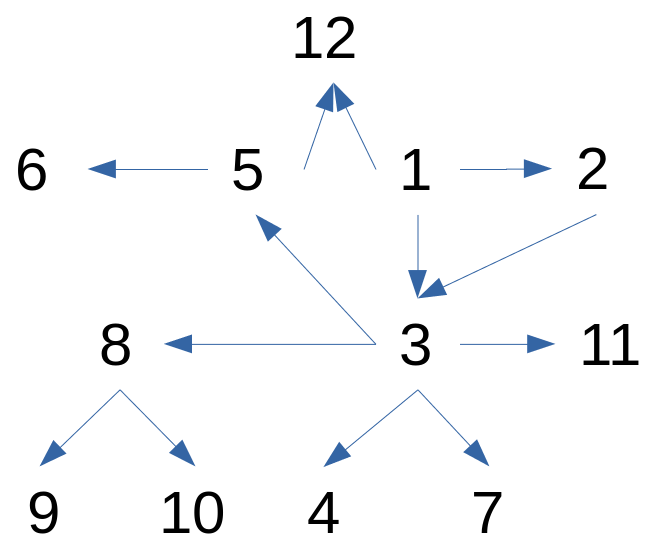
\includegraphics[width=3.0in]{relationship.png}
    \end{figure}

    \section{Verify the means, variances and MGFs of the rv.s given in Table 1.1 and Table 1.2 according to their PDFs/PMFs.}
    \begin{table}[h]
        \centering
        \caption{The PDF, mean, variance and MGF for some common continuous rv s}
        \begin{spacing}{2.0}
            \begin{tabular}{lllll}
                \hline
                Name & PDF $\text{f}_X(x)$ & Mean & Variance & MGF $\text{g}_X(r)$\\
                \hline
                Exponjential: & $\lambda\exp(-\lambda x);\quad x\geq0$ & $\frac{1}{\lambda}$ & $\frac{1}{\lambda^2}$ & $\frac{\lambda}{\lambda-r};\quad\text{for }r<\lambda$\\
                Erlang: & $\frac{\lambda^nx^{n-1}\exp(-\lambda x)}{(n-1)!};\quad x\geq0$ & $\frac{n}{\lambda}$ & $\frac{n}{\lambda^2}$ & $\big(\frac{\lambda}{\lambda-r}\big)^n;\quad\text{for }r<\lambda$\\
                Gaussian: & $\frac{1}{\sigma\sqrt{2\pi}}\exp\big(\frac{-(x-a)^2}{2\sigma^2}\big)$ & $a$ & $\sigma^2$ & $\exp(ra+r^2\sigma^2/2)$\\
                Uniform & $\frac{1}{a};\quad0\leq x\leq a$ & $\frac{a}{2}$ & $\frac{a^2}{12}$ & $\frac{\exp(ra)-1}{ra}$\\
                \hline
            \end{tabular}    
        \end{spacing}
    \end{table}


    \textbf{Solutions:}
    
    \begin{enumerate}
        \item Exponential
        \begin{equation*}
          \begin{split}
             E[X] & = \int_{0}^{\infty}\frac{\lambda x}{e^{\lambda x}}dx\\
               & = \frac{1}{\lambda}\int_{0}^{\infty}\frac{t}{e^t}dt,\quad\text{with $t=\lambda x$}\\
               &=\frac{-1}{\lambda}\int_{0}^{\infty}td(\frac{1}{e^t})\\
               & =\frac{-1}{\lambda}\bigg(\frac{t}{e^t}\bigg|^\infty_0-\int_{0}^{\infty}\frac{1}{e^t}dt\bigg)\\
               &=\frac{-1}{\lambda}[(0-0)-1]\\
               &=\frac{1}{\lambda}
          \end{split}
        \end{equation*}

        \begin{equation*}
          \begin{split}
             E[X^2] &=\frac{1}{\lambda^2}\int_{0}^{\infty}\frac{t^2}{e^t}dt,\quad\text{with $t=\lambda x$}\\
               &=\frac{-1}{\lambda^2}\int_{0}^{\infty}t^2d(\frac{1}{e^t})\\
               &=\frac{-1}{\lambda^2}\bigg(\frac{t^2}{e^t}\bigg|^\infty_0-2\int_{0}^{\infty}\frac{t}{e^t}dt\bigg)\\
               &=\frac{-1}{\lambda^2}[(0-0)-2]\quad\text{from equations above}\\
               &=\frac{2}{\lambda^2}
          \end{split}
        \end{equation*}

        Therefore, 
        \begin{equation*}
            \sigma^2_X= E[X^2]-(E[X])^2=\frac{1}{\lambda^2}
        \end{equation*}

        \begin{equation*}
          \begin{split}
             g_X(r)
               & =\lambda\int_{0}^{\infty}e^{(r-\lambda)x}dx\\
               & =\frac{\lambda}{r-\lambda}e^{(r-\lambda)x}\big|^\infty_0\\
               &=\frac{\lambda}{r-\lambda}(0-1),\quad\text{with $r<\lambda$, otherwise $\lim_{x\rightarrow\infty}e^{(r-\lambda)x}=\infty$}\\
               &=\frac{\lambda}{\lambda-r},\quad\text{with $r<\lambda$}
          \end{split}
        \end{equation*}
        The mean, varaince and MGF of the exponential distribution function has been derived.
        \item Erlang
            \begin{equation*}
                \begin{split}
                    E[X] &=\int_{0}^\infty\frac{(\lambda x)^{n}}{(n-1)!e^{\lambda x}}dx\\
                    &=\frac{1}{(n-1)!\lambda}\int_0^\infty\frac{t^n}{e^t}dt,\quad\text{with $t=\lambda x$}\\
                    &=\frac{-1}{(n-1)!\lambda}\int_0^\infty t^nd(\frac{1}{e^t})\\
                    &=\frac{-1}{(n-1)!\lambda}\bigg[\frac{t^n}{e^t}\bigg|^\infty_0-n\int^\infty_0\frac{t^{n-1}}{e^t}dt\bigg]\\
                    &=\frac{-1}{(n-1)!\lambda}\bigg[(0-0)-n\int^\infty_0\frac{t^{n-1}}{e^t}dt\bigg]\\
                    &=\frac{n}{(n-1)!\lambda}\int^\infty_0\frac{t^{n-1}}{e^t}dt\\
                    &=\vdots\quad\text{from the third equation above}\\
                    &=\frac{n}{\lambda}
                \end{split}
            \end{equation*}
            \begin{equation*}
                \begin{split}
                    E[X^2] &= \int^\infty_{0}\frac{\lambda^nx^{n+1}}{(n-1)!e^{\lambda x}}dx\\
                    &= \frac{1}{(n-1)!\lambda^2}\int_0^\infty\frac{t^{n+1}}{e^t}dt\\
                    &= \frac{1}{(n-1)!\lambda^2}\cdot(n+1)!\\
                    &= \frac{n^2+n}{\lambda^2}
                \end{split}
            \end{equation*}
            Therefore, 
            \begin{equation*}
                \sigma^2_X=E[X^2]-(E[X])^2=\frac{n^2+n}{\lambda^2}-\frac{n^2}{\lambda^2}=\frac{n}{\lambda^2}
            \end{equation*}

            \begin{equation*}
                \begin{split}
                    g_X(r) &=\int^\infty_{0}\frac{\lambda^nx^{n-1}e^{rx}}{(n-1)!e^{\lambda x}}dx\\
                    &=\frac{\lambda^n}{(n-1)!}\int^\infty_0x^{n-1}e^{(r-\lambda)x}dx\\
                    &=\frac{\lambda^n}{(n-1)!}\cdot\frac{1}{r-\lambda}\cdot\int^\infty_0x^{n-1}de^{(r-\lambda)x}\\
                    &=\frac{\lambda^n}{(n-1)!}\cdot\frac{1}{r-\lambda}\cdot\bigg[x^{n-1}e^{(r-\lambda)x}\bigg|^\infty_0-\int^\infty_0e^{(r-\lambda)x}d(x^{n-1})\bigg]\\
                    &=\frac{\lambda^n}{(n-1)!}\cdot\frac{1}{r-\lambda}\cdot[(0-0)-(n-1)\int^\infty_0x^{n-2}e^{(r-\lambda)x}dx]\\
                    & \qquad\qquad\qquad\text{with $r<\lambda$, otherwise $\lim_{x\rightarrow\infty}x^{n-1}e^{(r-\lambda)x}=\infty$}\\\
                    &= \frac{\lambda^n}{\lambda-r}\cdot\frac{1}{(n-2)!\cdot}\int^\infty_0x^{n-2}e^{(r-\lambda)x}dx\\
                    &=\vdots,\quad\text{from the third equation above}\\
                    &=\bigg(\frac{\lambda}{\lambda-r}\bigg)^n,\quad\text{with $r<\lambda$}
                \end{split}
            \end{equation*}

            The mean, varaince and MGF of the Erlang distribution function has been derived.
            \item Gaussian
            \begin{equation*}
                \begin{split}
                    E[X] &= \int_{-\infty}^\infty\frac{x}{\sigma\sqrt{2\pi}}e^{\frac{-(x-a)^2}{2\sigma^2}}dx\\
                    &=\frac{1}{\sigma\sqrt{2\pi}}\int^\infty_{-\infty}xe^{-(\frac{x-a}{\sqrt{2}\sigma})^2}dx \\
                    &=\frac{1}{\sqrt{\pi}}\int^\infty_{-\infty}\frac{\sqrt{2}\sigma t+a}{e^{t^2}}dt,\quad\text{with $t=\frac{x-a}{\sqrt{2}\sigma}$}\\
                    &=\frac{1}{\sqrt{\pi}}\bigg[\int^\infty_{-\infty}\frac{\sqrt{2}\sigma t}{e^{t^2}}dt+\int^\infty_{-\infty}\frac{a}{e^{t^2}}dt\bigg]\\
                    &=\frac{a}{\sqrt{\pi}}\int^\infty_{-\infty}\frac{1}{e^{t^2}}dt,\quad\text{since $f(t)=\frac{\sqrt{2}\sigma t}{e^{t^2}}$ is an odd function}\\
                    &=\frac{2a}{\sqrt{\pi}}\int^\infty_0\frac{1}{e^{t^2}}dt,\quad\text{since $f(t)=\frac{1}{e^{t^2}}$ is an even function}\\
                    &=\frac{2a}{\sqrt{\pi}}\cdot\frac{\sqrt{\pi}}{2}\\
                    &=a
                \end{split}
            \end{equation*}
            Note:
            \begin{equation*}
                (\int^\infty_0e^{-x^2}dx)^2=\int^\infty_0e^{-x^2}dx\int^\infty_0e^{-y^2}dy=\int^\infty_0\int^\infty_0e^{-(x^2+y^2)}dxdy
            \end{equation*}
            let $x=r\cos\theta$ and $y=r\sin\theta$, then
            \begin{equation*}
                \int^\infty_0\int^\infty_0e^{-(x^2+y^2)}dxdy=\int^{\frac{\pi}{2}}_0d\theta\int^\infty_0e^{-r^2}rdr=\int^{\frac{\pi}{2}}_0\frac{1}{2}d\theta=\frac{\pi}{4}
            \end{equation*}
            
            Therefore, $(\int^\infty_0e^{-x^2}dx)^2=\frac{\pi}{4}$ and $\int^\infty_0e^{-x^2}dx=\frac{\sqrt{\pi}}{2}$.

            \begin{equation*}
                \begin{split}
                    E[X^2] &= \int_{-\infty}^\infty\frac{x^2}{\sigma\sqrt{2\pi}}e^{\frac{-(x-a)^2}{2\sigma^2}}dx\\
                    &=\frac{1}{\sigma\sqrt{2\pi}}\int_{_\infty}^\infty x^2e^{-(\frac{x-a}{\sqrt{2}\sigma})^2}dx \\
                    &=\frac{1}{\sqrt{\pi}}\int^\infty_{-\infty}\frac{2\sigma^2t^2+2\sqrt{2}\sigma at+a^2}{e^{t^2}}dt\\
                    &=\frac{2\sigma^2}{\sqrt{\pi}}\int^\infty_{-\infty}\frac{t^2}{e^{t^2}}dt+\frac{2\sqrt{2}\sigma a}{\sqrt{\pi}}\int^\infty_{-\infty}\frac{t}{e^{t^2}}dt+\frac{a^2}{\sqrt{\pi}}\int^\infty_{-\infty}\frac{1}{e^{t^2}}dt\\
                    &= \frac{2\sigma^2}{\sqrt{\pi}}\int^\infty_{-\infty}\frac{t^2}{e^{t^2}}dt + 0 + a^2,\quad\text{since $f(t)=\frac{t}{e^{t^2}}$ is an odd function and use the fact before}\\
                    &=\frac{2\sigma^2}{\sqrt{\pi}}\int^\infty_{-\infty}\frac{t^2}{e^{t^2}}dt + a^2
                \end{split}
            \end{equation*}
            
            Then, 
            \begin{equation*}
                \begin{split}
                    \begin{split}
                        \int^\infty_{\infty}\frac{t^2}{e^{t^2}}dt &=2\int_0^\infty\frac{t^2}{e^{t^2}}dt,\quad\text{since $f(t)=\frac{t^2}{e^{t^2}}$ is an even function}\\
                         &=\int_0^\infty u^{\frac{1}{2}}e^{-u}du,\quad\text{with $u=t^2$}\\
                         &=\int_0^\infty u^{\frac{3}{2}-1}e^{-u}du\\
                         &=\Gamma(\frac{3}{2})=\frac{1}{2}\Gamma(\frac{1}{2})=\frac{\sqrt{\pi}}{2}
                    \end{split}
                \end{split}
            \end{equation*}

            
            \begin{equation*}
                \begin{split}
                    E(X^2)&=\frac{2\sigma^2}{\sqrt{\pi}}\int^\infty_{-\infty}\frac{t^2}{e^{t^2}}dt + a^2\\
                    &=\frac{2\sigma^2}{\sqrt{\pi}}\cdot\frac{\sqrt{\pi}}{2} +a^2\\
                    &=\sigma^2+a^2
                \end{split}
            \end{equation*}

            And
            \begin{equation*}
                \sigma^2_X=E[X^2]-(E[X])^2=\sigma^2+a^2-a^2=\sigma^2
            \end{equation*}

            \begin{equation*}
                \begin{split}
                    g_X(r)&=\int^\infty_{-\infty}\frac{1}{\sigma\sqrt{2\pi}}e^{rx}e^{\frac{-(x-a)^2}{2\sigma^2}}dx\\
                    &=\frac{1}{\sigma\sqrt{2\pi}}\int^\infty_{-\infty}e^{rx-(\frac{x-a}{\sqrt{2}\sigma})^2}dx\\
                    &=\frac{1}{\sqrt{\pi}}\int^{\infty}_{-\infty}e^{-(t^2-\sqrt{2}r\sigma t-ra)}dt,\quad\text{with $t=\frac{x-a}{\sqrt{2}\sigma}$}\\
                    &= \frac{e^{ra}}{\sqrt{\pi}}\int^\infty_{-\infty}e^{-(t^2-\sqrt{2}r\sigma t+\frac{r^2\sigma^2}{2})+\frac{r^2\sigma^2}{2}}dt\\
                    &= \frac{e^{ra+\frac{r^2\sigma^2}{2}}}{\sqrt{\pi}}\int^\infty_{-\infty}e^{-(t-\frac{\sqrt{2}}{2}r\sigma)}dt\\
                    &=\frac{e^{ra+\frac{r^2\sigma^2}{2}}}{\sqrt{\pi}}\int^\infty_{-\infty}e^{-u^2}du,\quad\text{with $u=t-\frac{\sqrt{2}}{2}r\sigma$}\\
                    &= \frac{e^{ra+\frac{r^2\sigma^2}{2}}}{\sqrt{\pi}}\cdot\sqrt{\pi},\quad\text{use the fact before}\\
                    &=e^{ra+\frac{r^2\sigma^2}{2}}
                \end{split}
            \end{equation*}

            Therefore, the mean, varaince and MGF of the Gaussian distribution function has been derived.
            \item Uniform
            \begin{equation*}
                \begin{split}
                    E[X] &= \int^a_0\frac{x}{a}dx\\
                        &= \frac{1}{2a}\cdot x^2\big|^a_0\\
                        &=\frac{a}{2}
                \end{split}
            \end{equation*}
            \begin{equation*}
                \begin{split}
                    E[X^2] &=\int^a_0\frac{x^2}{a}dx\\
                    &=\frac{1}{3a}\cdot x^3\big|^a_0\\
                    &=\frac{a^2}{3}
                \end{split}
            \end{equation*}

            Therefore, 
            \begin{equation*}
                \sigma^2_X=E[X^2]-(E[X])^2=\frac{a^2}{3}-\frac{a^2}{4}=\frac{a^2}{12}
            \end{equation*}
            
            \begin{equation*}
                \begin{split}
                    g_X(r)&=\int^a_0\frac{e^{rx}}{a}dx\\
                    &=\frac{1}{ra}\cdot e^{rx}\big|^a_0\\
                    &=\frac{e^{ra}-1}{ra}
                \end{split}
            \end{equation*}


            The mean, varaince and MGF of the uniform distribution function has been derived.
    \end{enumerate}

    \begin{table}[h]
        \centering
        \caption{The PMF, mean, variance and MGF for some common discrete rv s}
        \begin{spacing}{2.0}
            \begin{tabular}{lllll}
                \hline
                Name & PMF $\text{p}_M(m)$ & Mean & Variance & MGF $\text{g}_M(r)$\\
                \hline
                Binary: & $\text{p}_M(1)=p;\text{p}_M(0)=1-p$ & $p$ & $p(1-p)$ & $1-p+pe^r$\\
                Binomial & $\binom{n}{m}p^m(1-p)^{n-m};0\leq m\leq n$ & $np$ & $np(1-p)$ & $[1-p+pe^r]^n$\\
                Geometric & $p(1-p)^{m-1};m\geq1$ & $\frac{1}{p}$ & $\frac{1-p}{p^2}$ & $\frac{pe^r}{1-(1-p)e^r};\text{for }r<\ln\frac{1}{1-p}$\\
                Poisson: & $\frac{\lambda\exp(-\lambda)}{n!};n\geq0$ & $\lambda$ & $\lambda$ & $\exp[\lambda(e^r-1)]$\\
                \hline           
            \end{tabular}
        \end{spacing}
    \end{table}

    \textbf{Solutions:}
    \begin{enumerate}
        \item Binary
            \begin{equation*}
                \begin{split}
                    E[X] &= 1\cdot p+0\cdot(1-p)\\
                    &=p                    
                \end{split}            
            \end{equation*}
            \begin{equation*}
                \begin{split}
                    E[X^2] &= 1^2\cdot p+0^2\cdot(1-p)\\
                    &= p
                \end{split}
            \end{equation*}
        Then, 
            \begin{equation*}
                \sigma^2_X=E[X^2]-(E[X])^2=p(1-p)
            \end{equation*}
            
            \begin{equation*}
                \begin{split}
                    g_X(r) &= e^{r\cdot1}*p+e^{r\cdot0}(1-p)\\
                    &=1-p+pe^r
                \end{split}
            \end{equation*}
        \item Binomial
            \begin{equation*}
                \begin{split}
                    E[X] &=\sum^n_{k=0}k\cdot\binom{n}{k}p^k(1-p)^{n-k}\\
                    &=\sum^n_{k=1}k\cdot\frac{n!}{(n-k)!k!}p^k(1-p)^{n-k}\\
                    &=np\sum^n_{k=1}\frac{(n-1)!}{(n-k)!(k-1)!}p^{k-1}(1-p)^{n-k}\\
                    &=np\sum^{n}_{k=1}\frac{(n-1)!}{[(n-1)-(k-1)]!(k-1)!}p^{k-1}(1-p)^{[(n-1)-(k-1)]}\\
                    &=np\sum^{n}_{k=1}\binom{n-1}{k-1}p^{k-1}(1-p)^{[(n-1)-(k-1)]}\\
                    &=np\sum^{n-1}_{v=0}\binom{n-1}{v}p^v(1-p)^{(n-1)-v},\quad\text{with $v=k-1$}\\
                    &=np\sum^{u}_{v=0}\binom{u}{v}p^v(1-p)^{u-v},\quad\text{with $u=n-1$}\\
                    &=np(p+1-p)^u,\quad\text{according to the binomial theorem }\\
                    &=np
                \end{split}
            \end{equation*}

        \begin{equation*}
            \begin{split}
                E[X^2] &= \sum^n_{k=0}k^2\cdot\binom{n}{k}p^k(1-p)^{n-k}\\
                &= \sum^n_{k=1}k^2\cdot\frac{n!}{(n-k)!k!}p^k(1-p)^{n-k}\\
                &= np\sum^n_{k=1}k\cdot\frac{(n-1)!}{(n-k!)(k-1)!}p^{k-1}(1-p)^{n-k}\\
                &=np\sum^n_{k=1}k\cdot\frac{(n-1)!}{[(n-1)-(k-1)]!(k-1)!}p^{k-1}(1-p)^{(n-1)-(k-1)}\\
                &=np\sum^n_{k=1}k\cdot\binom{n-1}{k-1}p^k-1(1-p)^{(n-1)-(k-1)}\\
                &=np\sum^u_{v=0}(v+1)\binom{u}{v}p^v(1-p)^{u-v},\quad\text{with $u=n-1,v=k-1$}\\
                &=np\bigg[\sum^u_{v=0}v\binom{u}{v}p^v(1-p)^{u-v}+\sum^u_{v=0}\binom{u}{v}p^v(1-p)^{u-v}\bigg]\\
                &=np(up+(p+1-p)^u),\quad\text{use the facts before}\\
                &=np[(n-1)p+1]\\
                &=n^2p^2+np(1-p)
            \end{split}
        \end{equation*}

        Then,
        \begin{equation*}
            \sigma^2_X=E[X^2]-(E[X])^2=n^2p^2+np(1-p)-n^2p^2=np(1-p)
        \end{equation*}

        \begin{equation*}
            \begin{split}
                g_X(r) &= \sum^n_{k=0}e^{rk}\cdot\binom{n}{k}p^k(1-p)^{n-k}\\
                &=\sum^n_{k=0}\binom{n}{k}(pe^r)^k(1-p)^{n-k}\\
                &=(1-p+pe^r)^n,\quad\text{according to the binomial theorem}
            \end{split}
        \end{equation*}

        \item Geometric
        let $q=1-p$, then 
        \begin{equation*}
            \begin{split}
                E[X] &=\sum^\infty_{k=1}kpq^{k-1}\\
                &=p\sum^\infty_{k=1}kq^{k-1}\\
                &=p\frac{d(\sum^\infty_{k=1}q^k)}{dq}\\
                &=p\frac{d(\sum^\infty_{t=0}q^t)}{dq}\\
                &=p\frac{d}{dq}(\frac{1}{1-q})\\
                &=p\frac{1}{(1-q)^2}\\
                &=\frac{1}{p}
            \end{split}
        \end{equation*}

        \begin{equation*}
            \begin{split}
                E[X^2] &= \sum^\infty_{k=1}k^2pq^{k-1}\\
                &=p\bigg[\sum^\infty_{k=1}k(k-1)q^{k-1}+\sum^\infty_{k=1}kq^{k-1}\bigg]\\
                &=p\bigg[\sum^\infty_{k=1}k(k-1)q^{k-1}+\frac{1}{p^2}\bigg],\quad\text{from the fact before}
            \end{split}
        \end{equation*}

        Since,
        \begin{equation*}
            \begin{split}
                \sum^\infty_{k=1}k(k-1)q^{k-1} & =q\sum^\infty_{k=1}k(k-1)q^{k-2}\\
                &= q\frac{d^2}{dq^2}\sum^\infty_{k=0}q^k\\
                &=\frac{2q}{p^3}
            \end{split}
        \end{equation*}
        
        Therefore,
        \begin{equation*}
            \begin{split}
                E[X^2] &= p(\frac{2q}{p^3}+\frac{1}{p^2})\\
                &=\frac{2q}{p^2}+\frac{1}{p}\\
                &=\frac{2-p}{p^2}
            \end{split}
        \end{equation*}
        
        And
        \begin{equation*}
            \sigma^2_X=E[X^2]-(E[X])^2=\frac{2-p}{p}-\frac{1}{p^2}=\frac{1-p}{p^2}
        \end{equation*}

        \begin{equation*}
            \begin{split}
                g_M(r) &= \sum^\infty_{k=1}pe^{rk}(1-p)^{k-1}\\
                &=\frac{p}{1-p}\sum^\infty_{k=1}e^{rk}(1-p)^{k}\\
                &=\frac{p}{1-p}\sum^\infty_{k=1}[(1-p)e^r]^k\\
                &=\frac{p}{1-p}\cdot\lim_{n\rightarrow\infty}\frac{(1-p)e^r\big(1-[(1-p)e^r)]\big)^n}{1-(1-(1-p)e^r}\\
                &=\frac{p}{1-p}\frac{(1-p)e^r}{1-(1-p)e^r},\quad\text{with $(1-p)e^r<1$ to be convergent}\\
                &=\frac{pe^r}{1-(1-p)e^r},\quad\text{with $r<\ln\frac{1}{1-p}$}
            \end{split}            
        \end{equation*}
        \item Poisson
            \begin{equation*}
                \begin{split}
                    E[X] &= \sum^\infty_{k=0}\frac{k\lambda^k}{k!e^\lambda}\\
                    &=\frac{1}{e^\lambda}\sum^\infty_{k=1}\frac{k\lambda^k}{k!}\\
                    &=\frac{\lambda}{e^\lambda}\sum^\infty_{k=1}\frac{\lambda^{k-1}}{(k-1)!}\\
                    &=\frac{\lambda}{e^\lambda}\sum^\infty_{n=0}\frac{\lambda^n}{n!}\\
                    &=\frac{\lambda}{e^\lambda}\cdot e^\lambda\\
                    &=\lambda
                \end{split}
            \end{equation*}
            \begin{equation*}
                \begin{split}
                    E[X^2] &=\sum^\infty_{k=0}\frac{k^2\lambda^k}{k!e^\lambda}\\
                    &=\frac{1}{e^\lambda}\sum^\infty_{k=1}\frac{k^2\lambda^k}{k!}\\
                    &=\frac{\lambda}{e^\lambda}\sum^\infty_{k=1}\frac{k\lambda^k}{(k-1)!}\\
                    &=\frac{\lambda}{e^\lambda}\sum^\infty_{n=0}\frac{(n+1)\lambda^n}{n!}\\
                    &=\frac{\lambda}{e^\lambda}\bigg[\sum^\infty_{n=0}\frac{n\lambda^n}{n!}+\sum^\infty_{n=0}\frac{\lambda^n}{n!}\bigg]\\
                    &=\frac{\lambda}{e^\lambda}[\lambda e^\lambda+e^\lambda],\quad\text{use the facts before}\\
                    &=\lambda^2+\lambda
                \end{split}
            \end{equation*}
        Then,
        \begin{equation*}
            \sigma^2_X=E[X^2]-(E[X])^2=\lambda^2+\lambda-\lambda^2=\lambda
        \end{equation*}
        
        \begin{equation*}
            \begin{split}
                g_X(r) &=\sum^\infty_{k=0}\frac{\lambda^k e^{rk}}{k!e^\lambda}\\
                &=\frac{1}{e^\lambda}\sum^\infty_{k=0}\frac{(\lambda e^r)^k}{k!}\\
                &=\frac{1}{e^\lambda}\cdot e^{\lambda e^r}\\
                &=\exp[\lambda(e^r-1)]
            \end{split}
        \end{equation*}
    \end{enumerate}
\end{document}